\documentclass[12pt]{article}
\usepackage{ragged2e} 
\usepackage{hyperref}
\usepackage[T1]{fontenc}

\hypersetup{
    colorlinks=true,
    linkcolor=orange!80!black,
    urlcolor=blue,  
    citecolor=blue, 
}

\usepackage[utf8]{inputenc}

\usepackage{pgfplots}
\usepackage{tikz}
\usepackage{pgf-pie}
\usetikzlibrary{pgfplots.statistics}

\usepackage{filecontents}
\usepackage{multirow}
\usepackage{amsmath}
\pgfplotsset{width=10cm,compat=1.17}
\setlength{\parskip}{0.75em} % Spacing between paragraphs
\usepackage{setspace}
\setstretch{1.2} % Adjust the value as per preference
\usepackage[margin=2cm]{geometry} % Adjust the margin
\setlength{\parindent}{0pt} % Adjust value for starting paragraph

\usepackage{mdframed}
\usepackage{float}

\usepackage{xcolor}
\usepackage{titlesec}
\usepackage{titletoc}
\usepackage{listings}
\usepackage{tcolorbox}
\usepackage{lipsum} % Example text package
\usepackage{fancyhdr} % Package for customizing headers and footers

% Define the orange color RGB
\definecolor{myorange}{RGB}{255,65,0}
% Define a new color for "cherry" (dark red)
\definecolor{cherry}{RGB}{148,0,25}
\definecolor{codegreen}{rgb}{0,0.6,0}

%%%%%%%%%%%%%%%%%%%%%%%%%%%%%%%%%%%%%%%%%%%%%%%%%%%%%%%%%%%%%%%%%%%%%
% Apply the custom footer to each page
\fancyhf{} % Clear all header and footer fields
\renewcommand{\headrulewidth}{0pt} % Remove header rule

%%%%%%%%%%%%%%%%%%%%%%%%%%%%%%%%%%%%%%%%%%%%%%%%%%%%%%%%%%%%%%%%%%%%%

% Set the color for the section headings
\titleformat{\section}
{\normalfont\Large\bfseries\color{orange!80!black}}{\thesection}{1em}{}

% Set color for the subsection headings
\titleformat{\subsection}
{\normalfont\large\bfseries\color{orange!80!black}}{\thesubsection}{1em}{}

% Set color for the subsubsection headings
\titleformat{\subsubsection}
{\normalfont\normalsize\bfseries\color{orange!80!black}}{\thesubsubsection}{1em}{}

%%%%%%%%%%%%%%%%%%%%%%%%%%%%%%%%%%%%%%%%%%%%%%%%%%%%%%%%%%%%%%%%%%%%%
% Set color for the table of contents
\titlecontents{section}
[1.5em]{\color{orange!80!black}}
{\contentslabel{1.5em}}
{}{\titlerule*[0.5pc]{.}\contentspage}

% Set the color for the subsections in the table of contents
\titlecontents{subsection}
[3.8em]{\color{orange!80!black}}
{\contentslabel{2.3em}}
{}{\titlerule*[0.5pc]{.}\contentspage}

% Set the color for the subsubsections in the table of contents
\titlecontents{subsubsection}
[6em]{\color{orange!80!black}}
{\contentslabel{3em}}
{}{\titlerule*[0.5pc]{.}\contentspage}

%%%%%%%%%%%%%%%%%%%%%%%%%%%%%%%%%%%%%%%%%%%%%%%%%%%%%%%%%%%%%%%%%%%%%
% set a format for C Code format
\lstset{
    language=C,
    basicstyle=\ttfamily,
    backgroundcolor=\color{blue!5},
    keywordstyle=\color{blue},
    commentstyle=\color{codegreen},
    stringstyle=\color{red},
    showstringspaces=false,
    breaklines=true,
    frame=single,
    rulecolor=\color{lightgray!35}, % Set the color of the frame
    numbers=none,
    numberstyle=\tiny,
    numbersep=5pt,
    tabsize=1,
    alsoletter={\#},
    otherkeywords={\#}
}

\lstdefinestyle{latexstyle}{
    language={[LaTeX]TeX},
    basicstyle=\ttfamily,
    backgroundcolor=\color{blue!5},
    keywordstyle=\color{blue},
    commentstyle=\color{codegreen},
    stringstyle=\color{red},
    showstringspaces=false,
    breaklines=true,
    frame=single,
    rulecolor=\color{lightgray!35}, % Set the color of the frame
    numbers=none,
    numberstyle=\tiny,
    numbersep=5pt,
    tabsize=1,
    morekeywords={documentclass, usepackage, begin, end},
}

% Define a command for inline code snippets with a colored and rounded box
\newtcbox{\codebox}[1][gray]{on line, boxrule=0.2pt, colback=blue!5, colframe=#1, fontupper=\color{cherry}\ttfamily, arc=2pt, boxsep=0pt, left=2pt, right=2pt, top=3pt, bottom=2pt}

%%%%%%%%%%%%%%%%%%%%%%%%%%%%%%%%%%%%%%%%%%%%%%%%%%%%%%%%%%%%%%%%%%%%%

% Define a new tcolorbox style with default options for sections called Tips!
\tcbset{
    myboxstyle/.style={
        colback=orange!10,
        colframe=orange!80!black,
    }
}

% Define a new tcolorbox style with default options to print the output with terminal style
\tcbset{
    myboxstyleTerminal/.style={
        colback=blue!5,
        frame empty, % Set frame to empty to remove the fram
    }
}

\mdfdefinestyle{myboxstyleTerminal1}{
    backgroundcolor=blue!5,
    hidealllines=true, % Remove all lines (frame)
    leftline=false,     % Add a left line
}

\title{ \\ \Large \textbf{Arduino Maze Game}}
\author{George Ghiugan}
\date{January 30, 2023}

\begin{document}
%%%%%%%%%%%%%%%%%%%%%%%%%%%%%%%%%%%%%%%%%%%%%%%%%%%%%%%%%%%%%%%%%%%%%%%%%%%%%%%%%%%%%%%%%%%%%%%%%%%%%%%%%%%%%%%%%%%%%%%%%%%%%%%%%%
\maketitle

\begin{figure}[H]
    \centering
    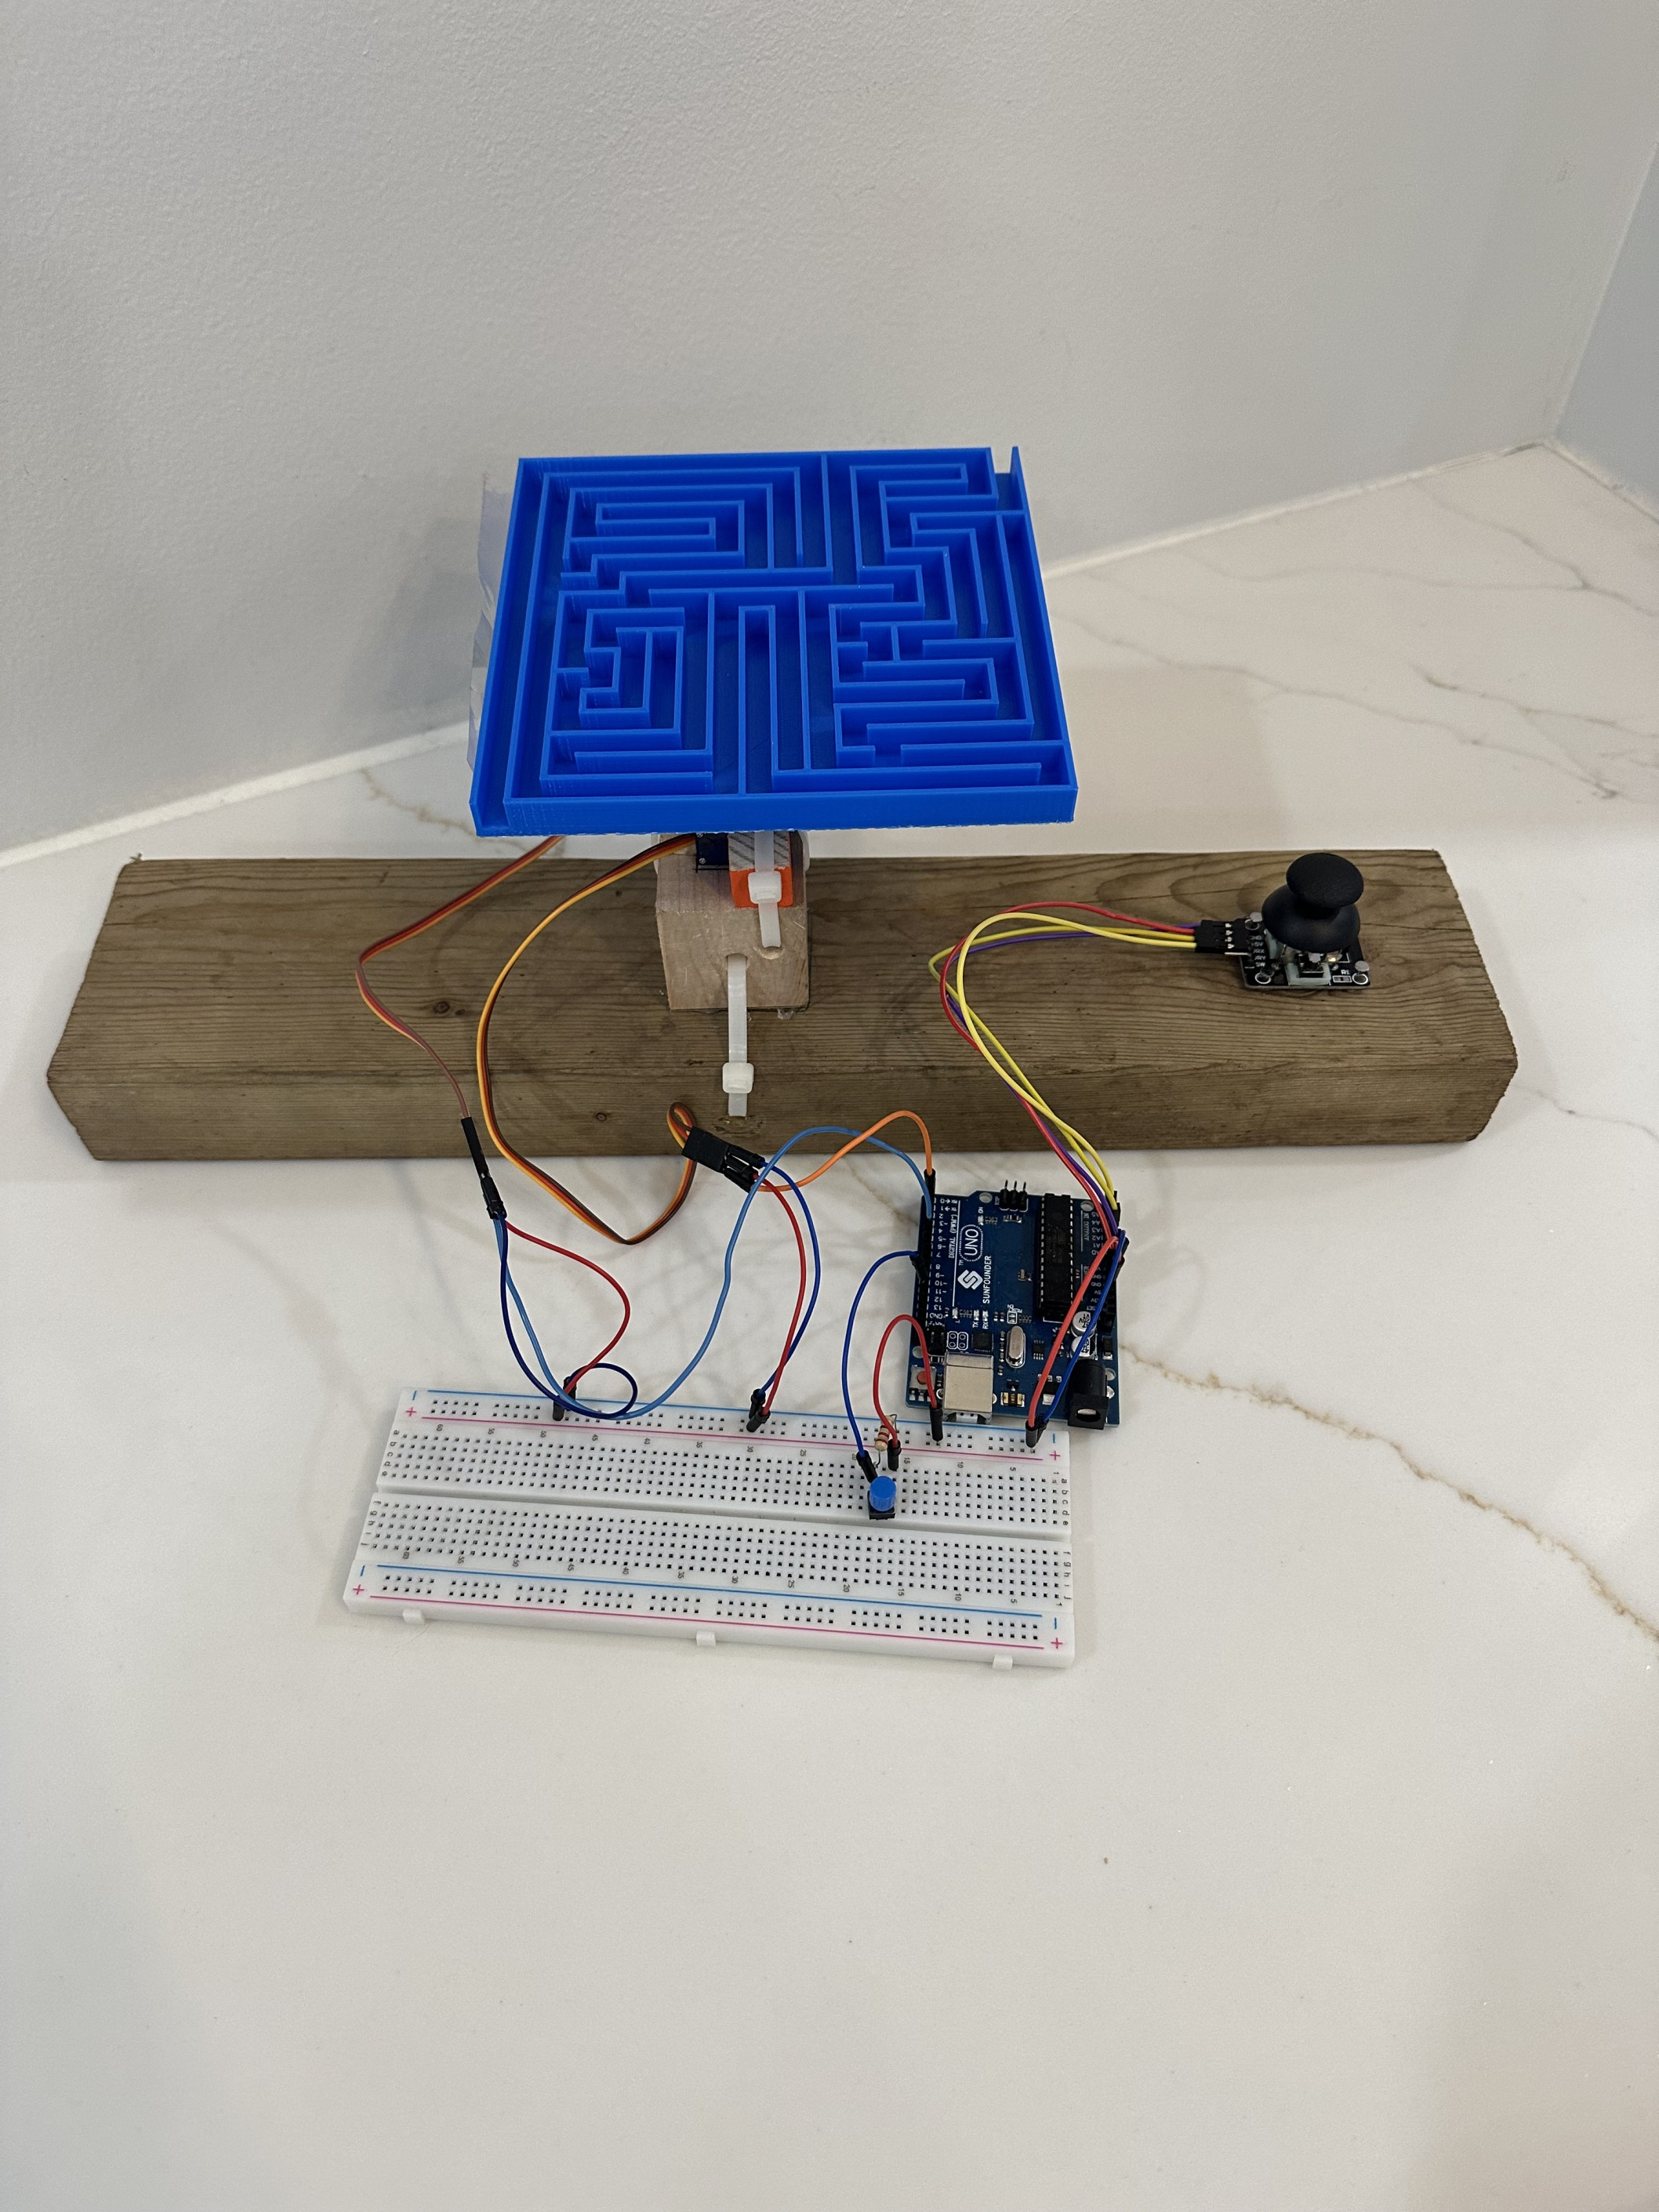
\includegraphics[width=0.7\linewidth]{image.jpg}
    \caption{Final Product}
    \label{fig:enter-label}
\end{figure}

\section*{Description:}

The Arduino Maze game is an engaging game which allows individuals to practice and develop their fine motor skills in an entertaining manner. The inspiration of making this project was to create a product which would assist patients in their development/rehabilitation of fine motor skills. The applications of creating this product is one which allows patients of all demographics to utilize this game for their well-being. For example healthcare providers are able to use the principles of my game in order to test patients fine motor skills over time and use it for analysis and diagnosis purposes of coordination affected disorders such as Parkinson's Disease. Overall, the Arduino Maze game can be used both in a fun manner to test your skills and for training of fine motor skills.


\section*{How to play:}
Use the joystick to control the movement of the maze. Maneuver the ball throughout the maze and solve it. For more of a challenge press and hold the blue button to increase the sensitivity of the joystick controlling the maze.

\section*{Process:}

\begin{figure}[H]
    \centering
    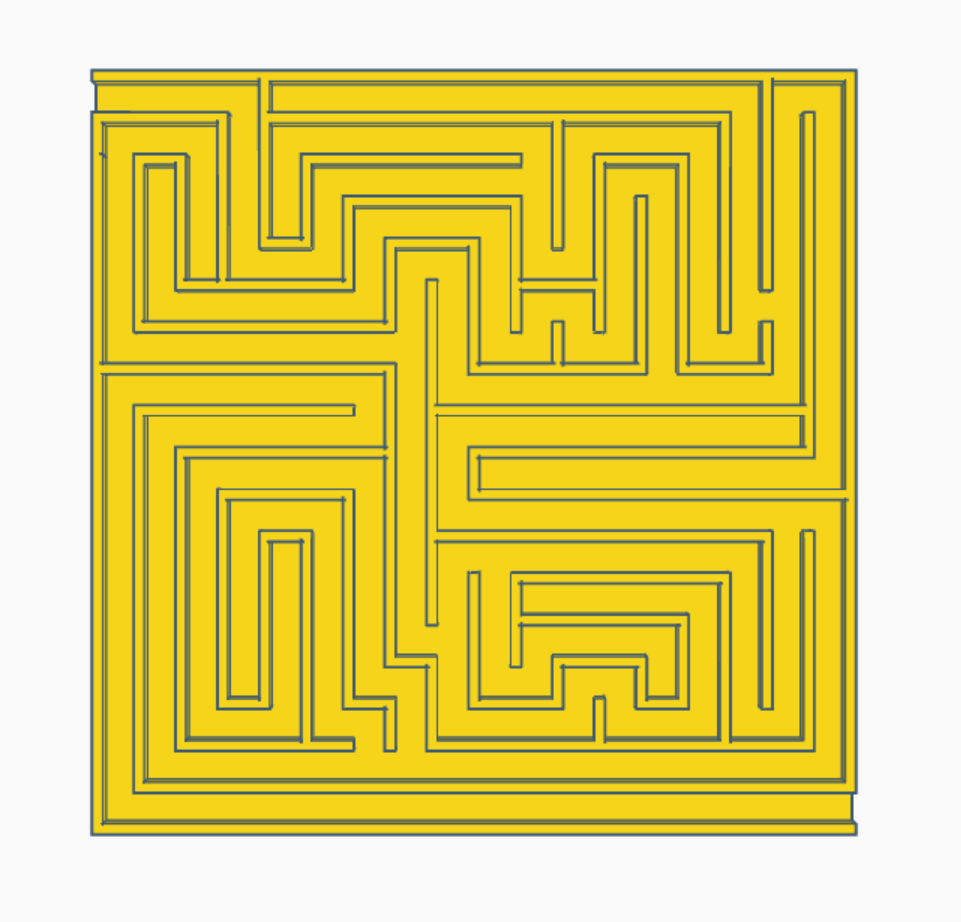
\includegraphics[width=0.5\linewidth]{topView3d.png}
    \caption{TinkerCAD Maze}
    \label{fig:enter-label}
\end{figure}

\vspace*{0.5cm} % Adjust the value as needed
\begin{figure}[H]
    \centering
    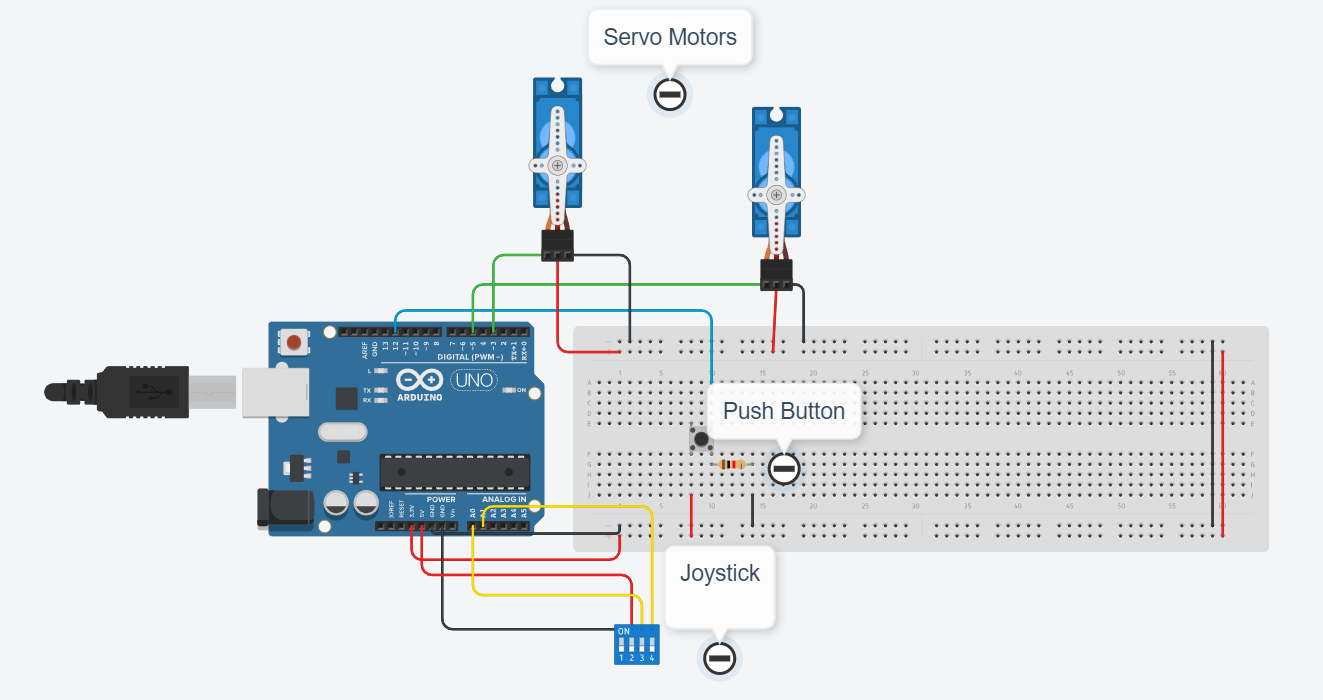
\includegraphics[width=1\linewidth]{tinkerMaze.png}
    \caption{TinkerCAD Circuit}
    \label{fig:enter-label}
\end{figure}



% The itemize list for each image
\begin{itemize}
    \item First step was to design the components/maze using TinkerCAD
    \item One servo motor controls the x-axis movement and one servo for the y-axis movement
  \end{itemize}

  \begin{figure}[H]
    \centering
    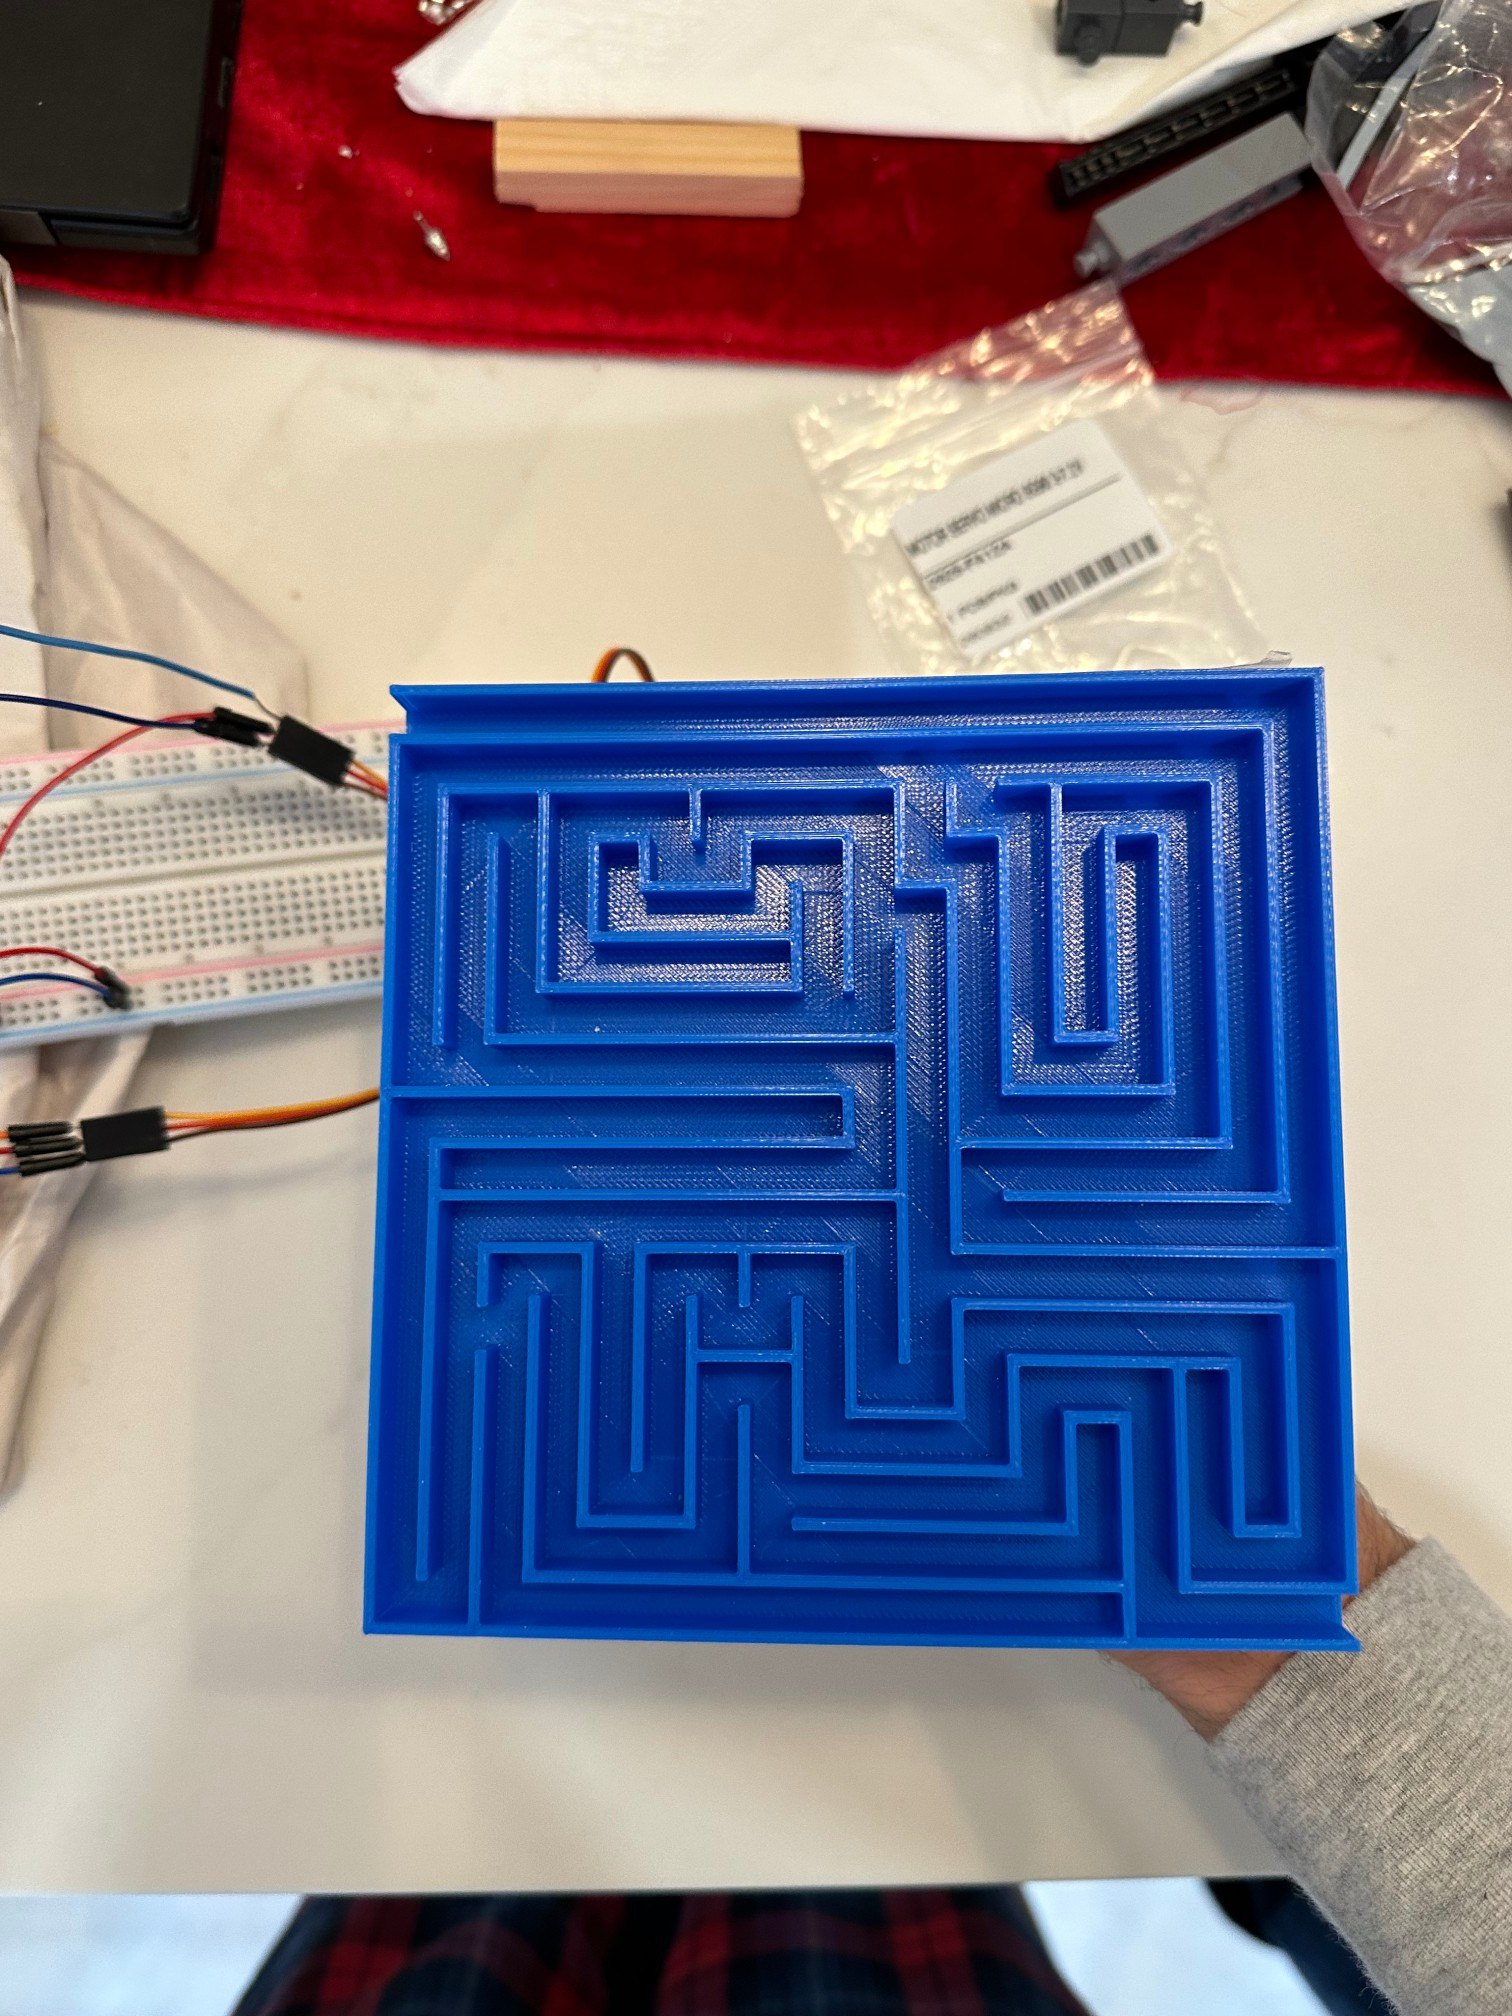
\includegraphics[width=0.7\linewidth]{IMG_0308.jpg}
    \caption{3d printed maze}
    \label{fig:enter-label}
\end{figure}

\begin{itemize}
  \item The final 3d printed maze
\end{itemize}

\begin{figure}[H]
    \centering
    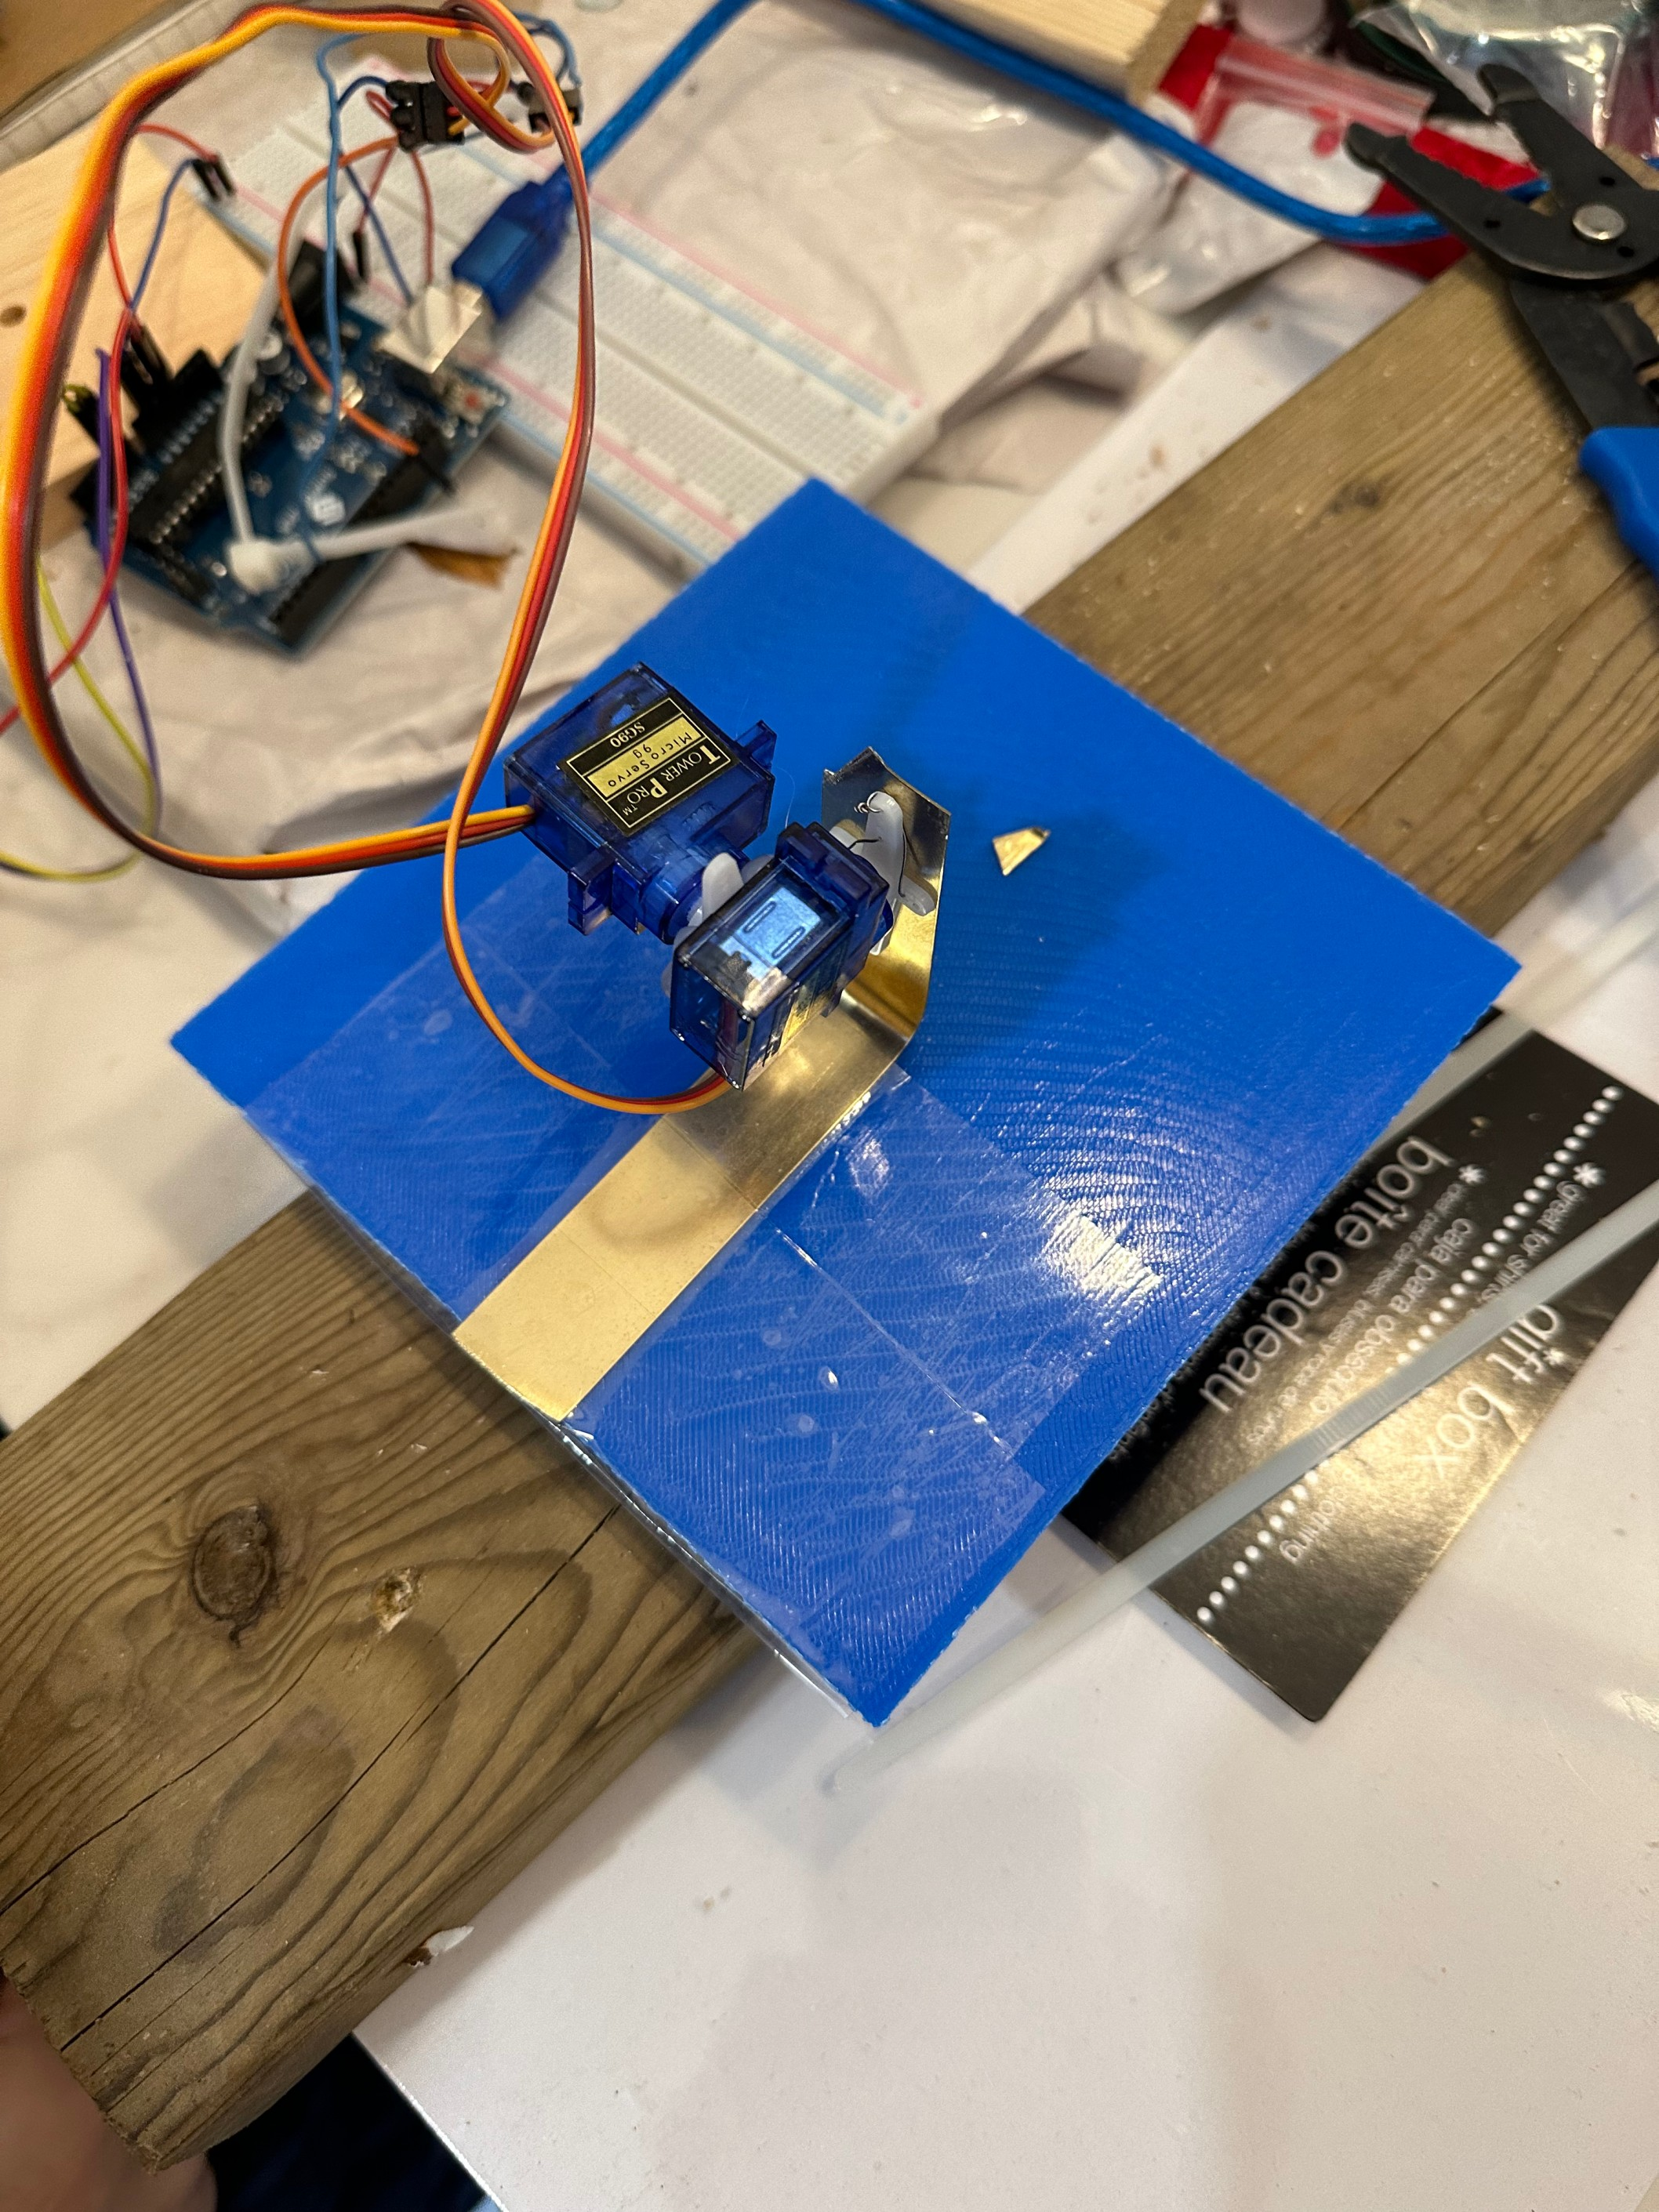
\includegraphics[width=0.7\linewidth]{IMG_0315.jpg}
    \caption{Servo Motor Attachment}
    \label{fig:enter-label}
\end{figure}

\begin{itemize}
    \item The installation of the two servo motors onto the maze
    \item Used a malleable metal to bend it in an L-shape
    \item Attached one servo with wires on the metal and the other superglued onto the servo
    \item Tested the movement to make sure it covers the entire x and y plane with the joystick
  \end{itemize}

\begin{figure}[H]
    \centering
    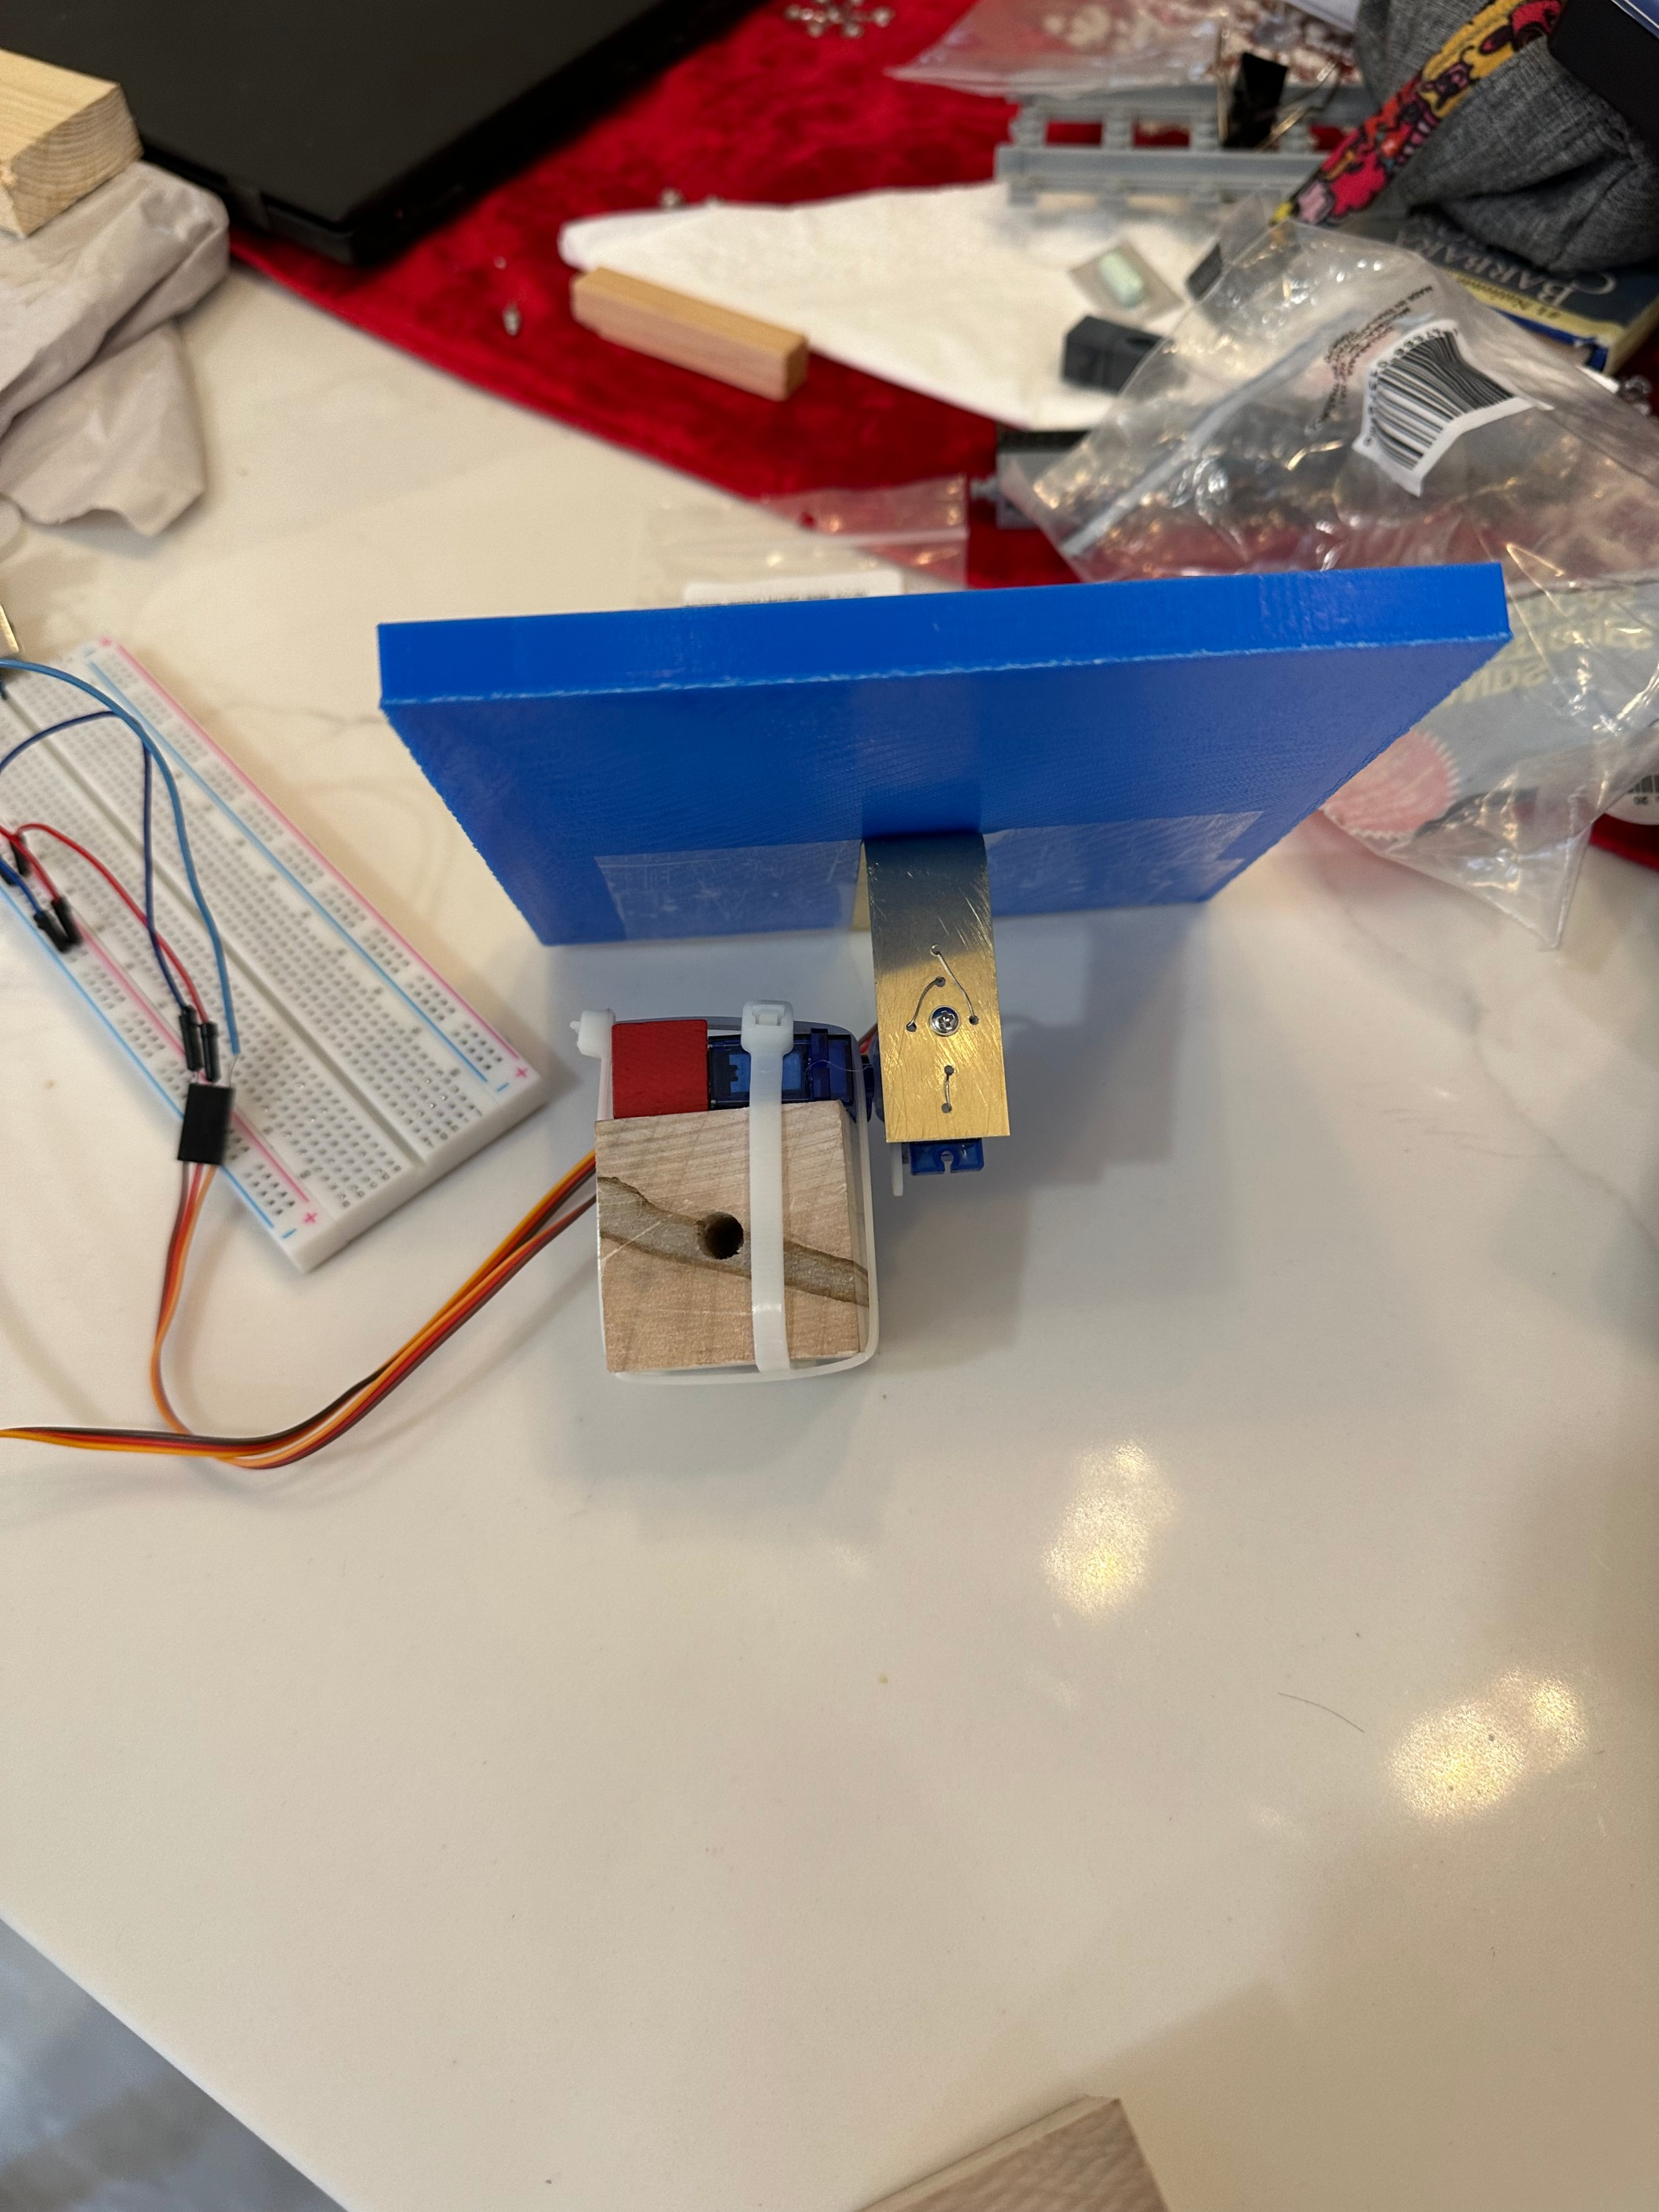
\includegraphics[width=0.7\linewidth]{IMG_0311.jpg}
    \caption{Maze Foundation Assembly}
    \label{fig:enter-label}
\end{figure}

\begin{itemize}
    \item Added a wooden block to secure the servo structures firmly
    \item Used 2 zip ties to firmly secure the servo motors
  \end{itemize}

\begin{figure}[H]
    \centering
    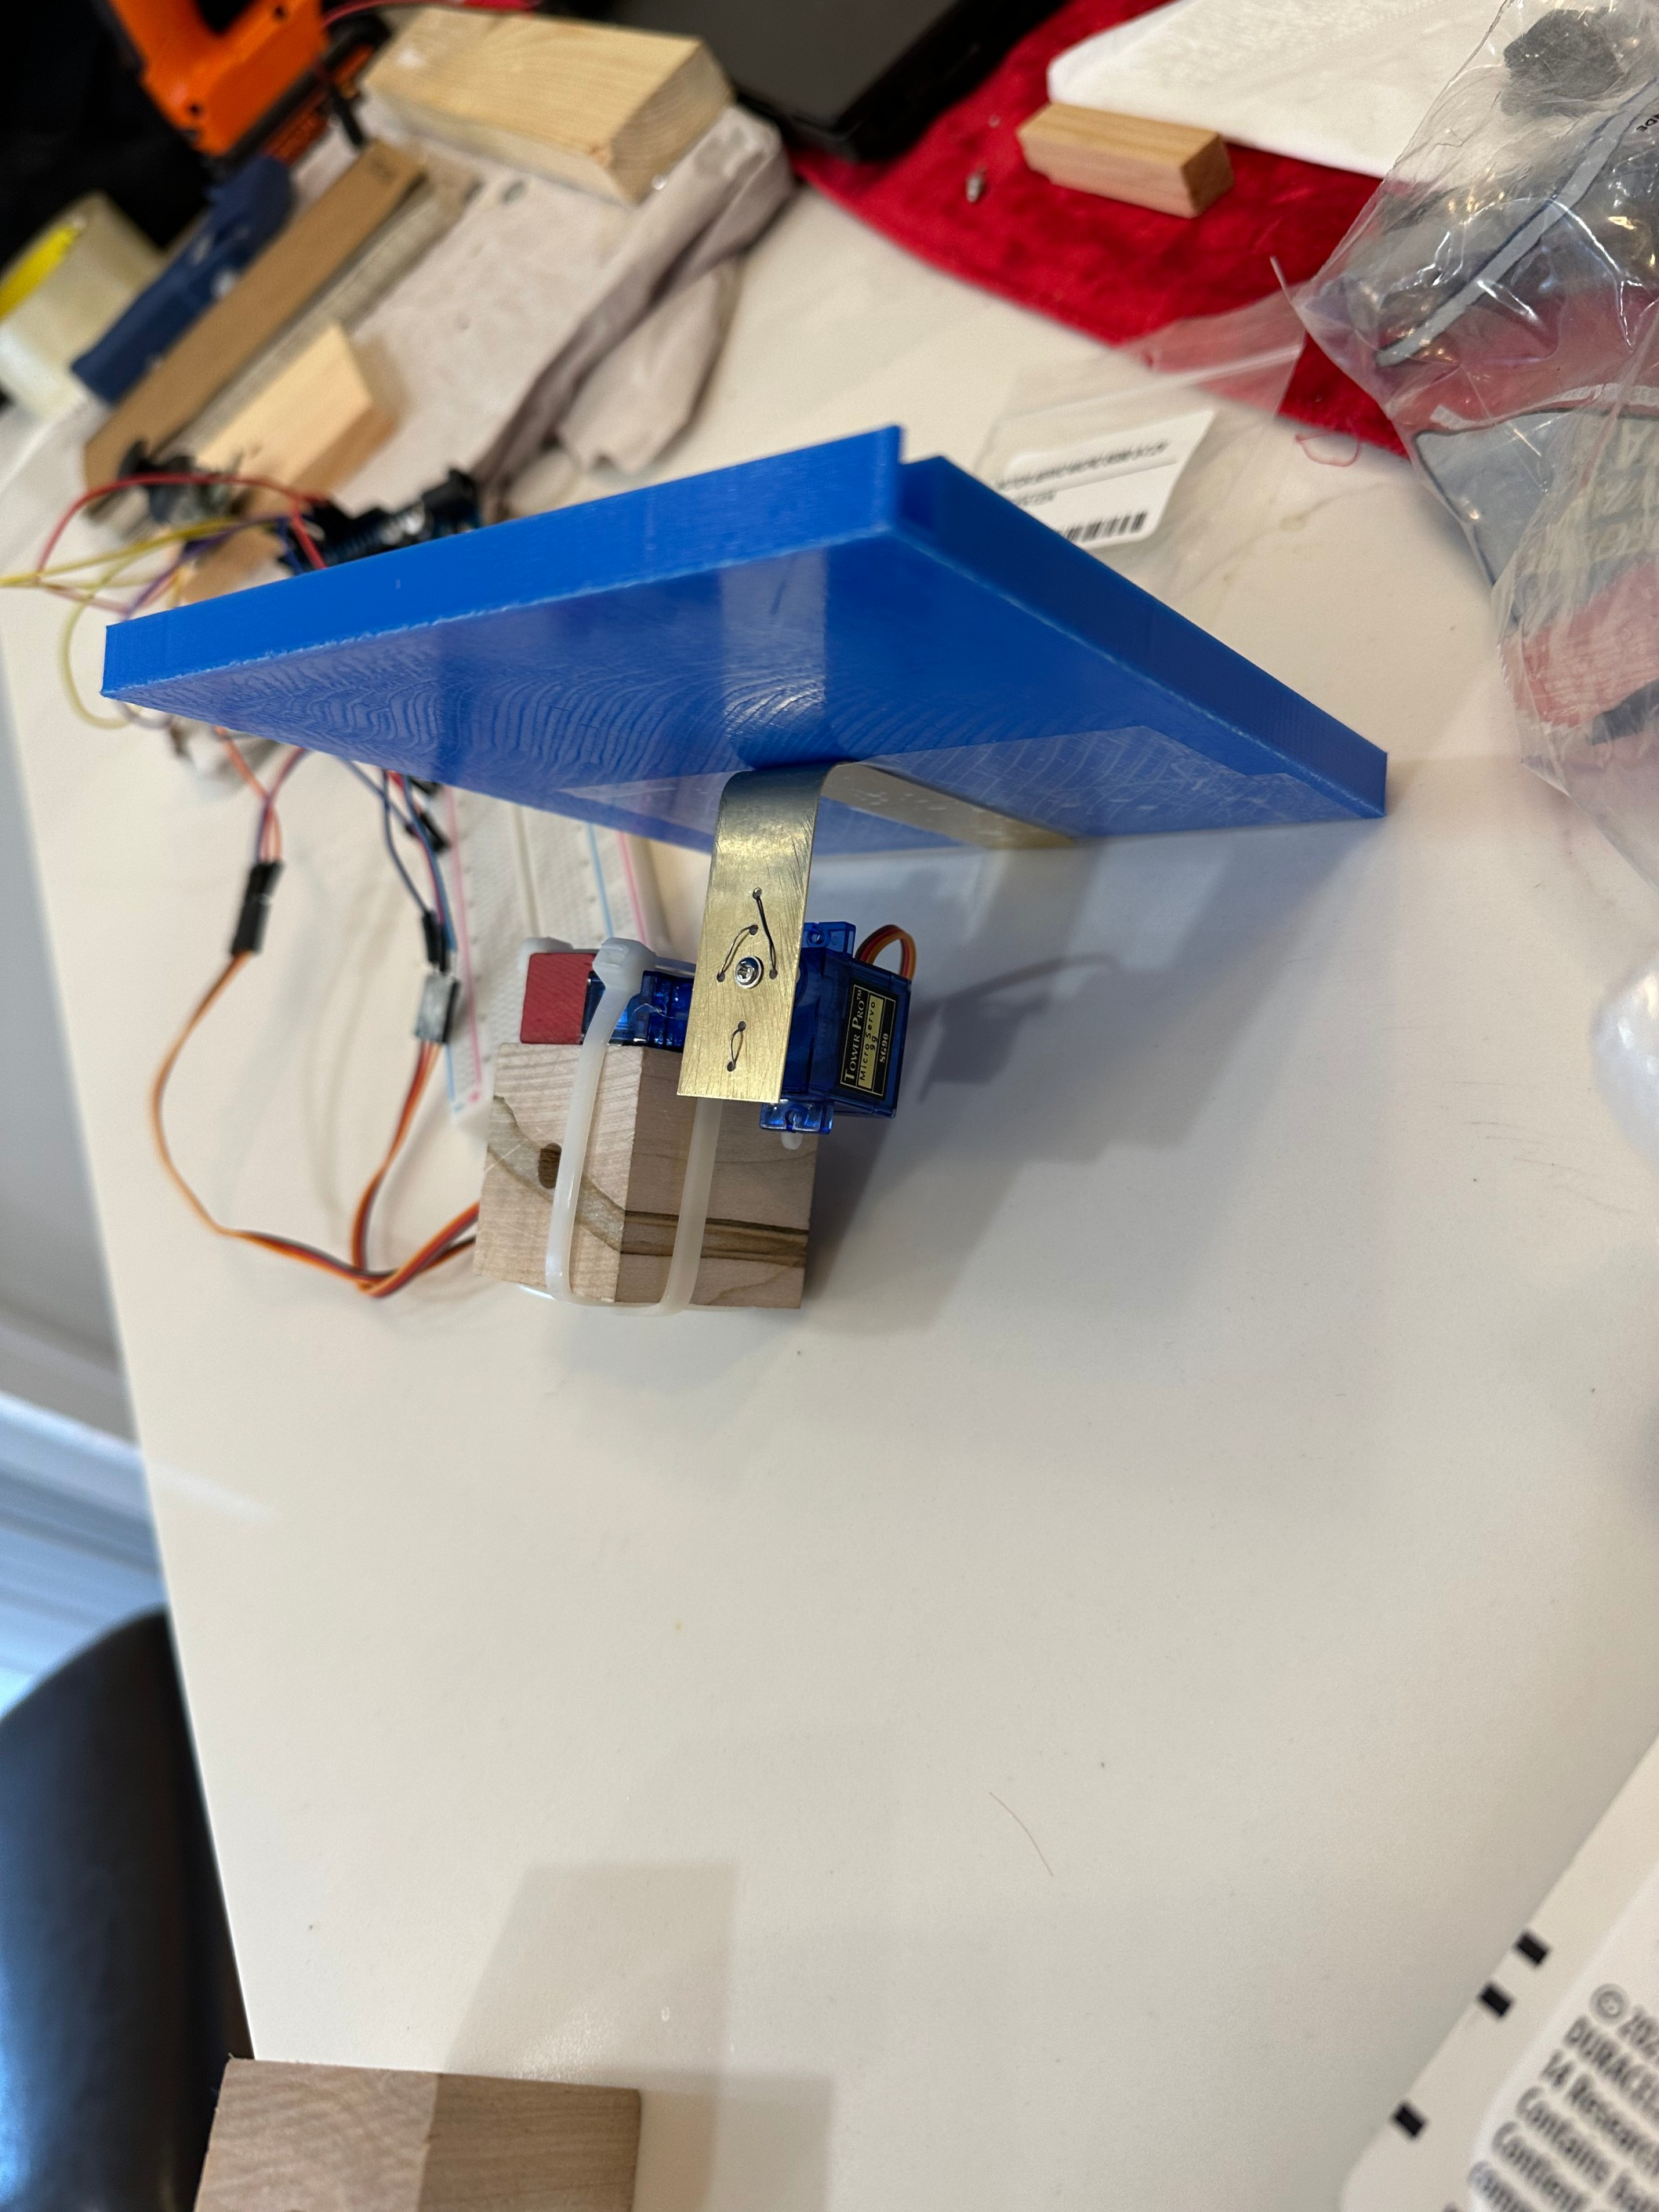
\includegraphics[width=0.7\linewidth]{IMG_0312.jpg}
    \caption{Maze Foundation Assembly Side View}
    \label{fig:enter-label}
\end{figure}

\begin{itemize}
    \item Side view of the wooden block supported structure 
  \end{itemize}

\begin{figure}[H]
    \centering
    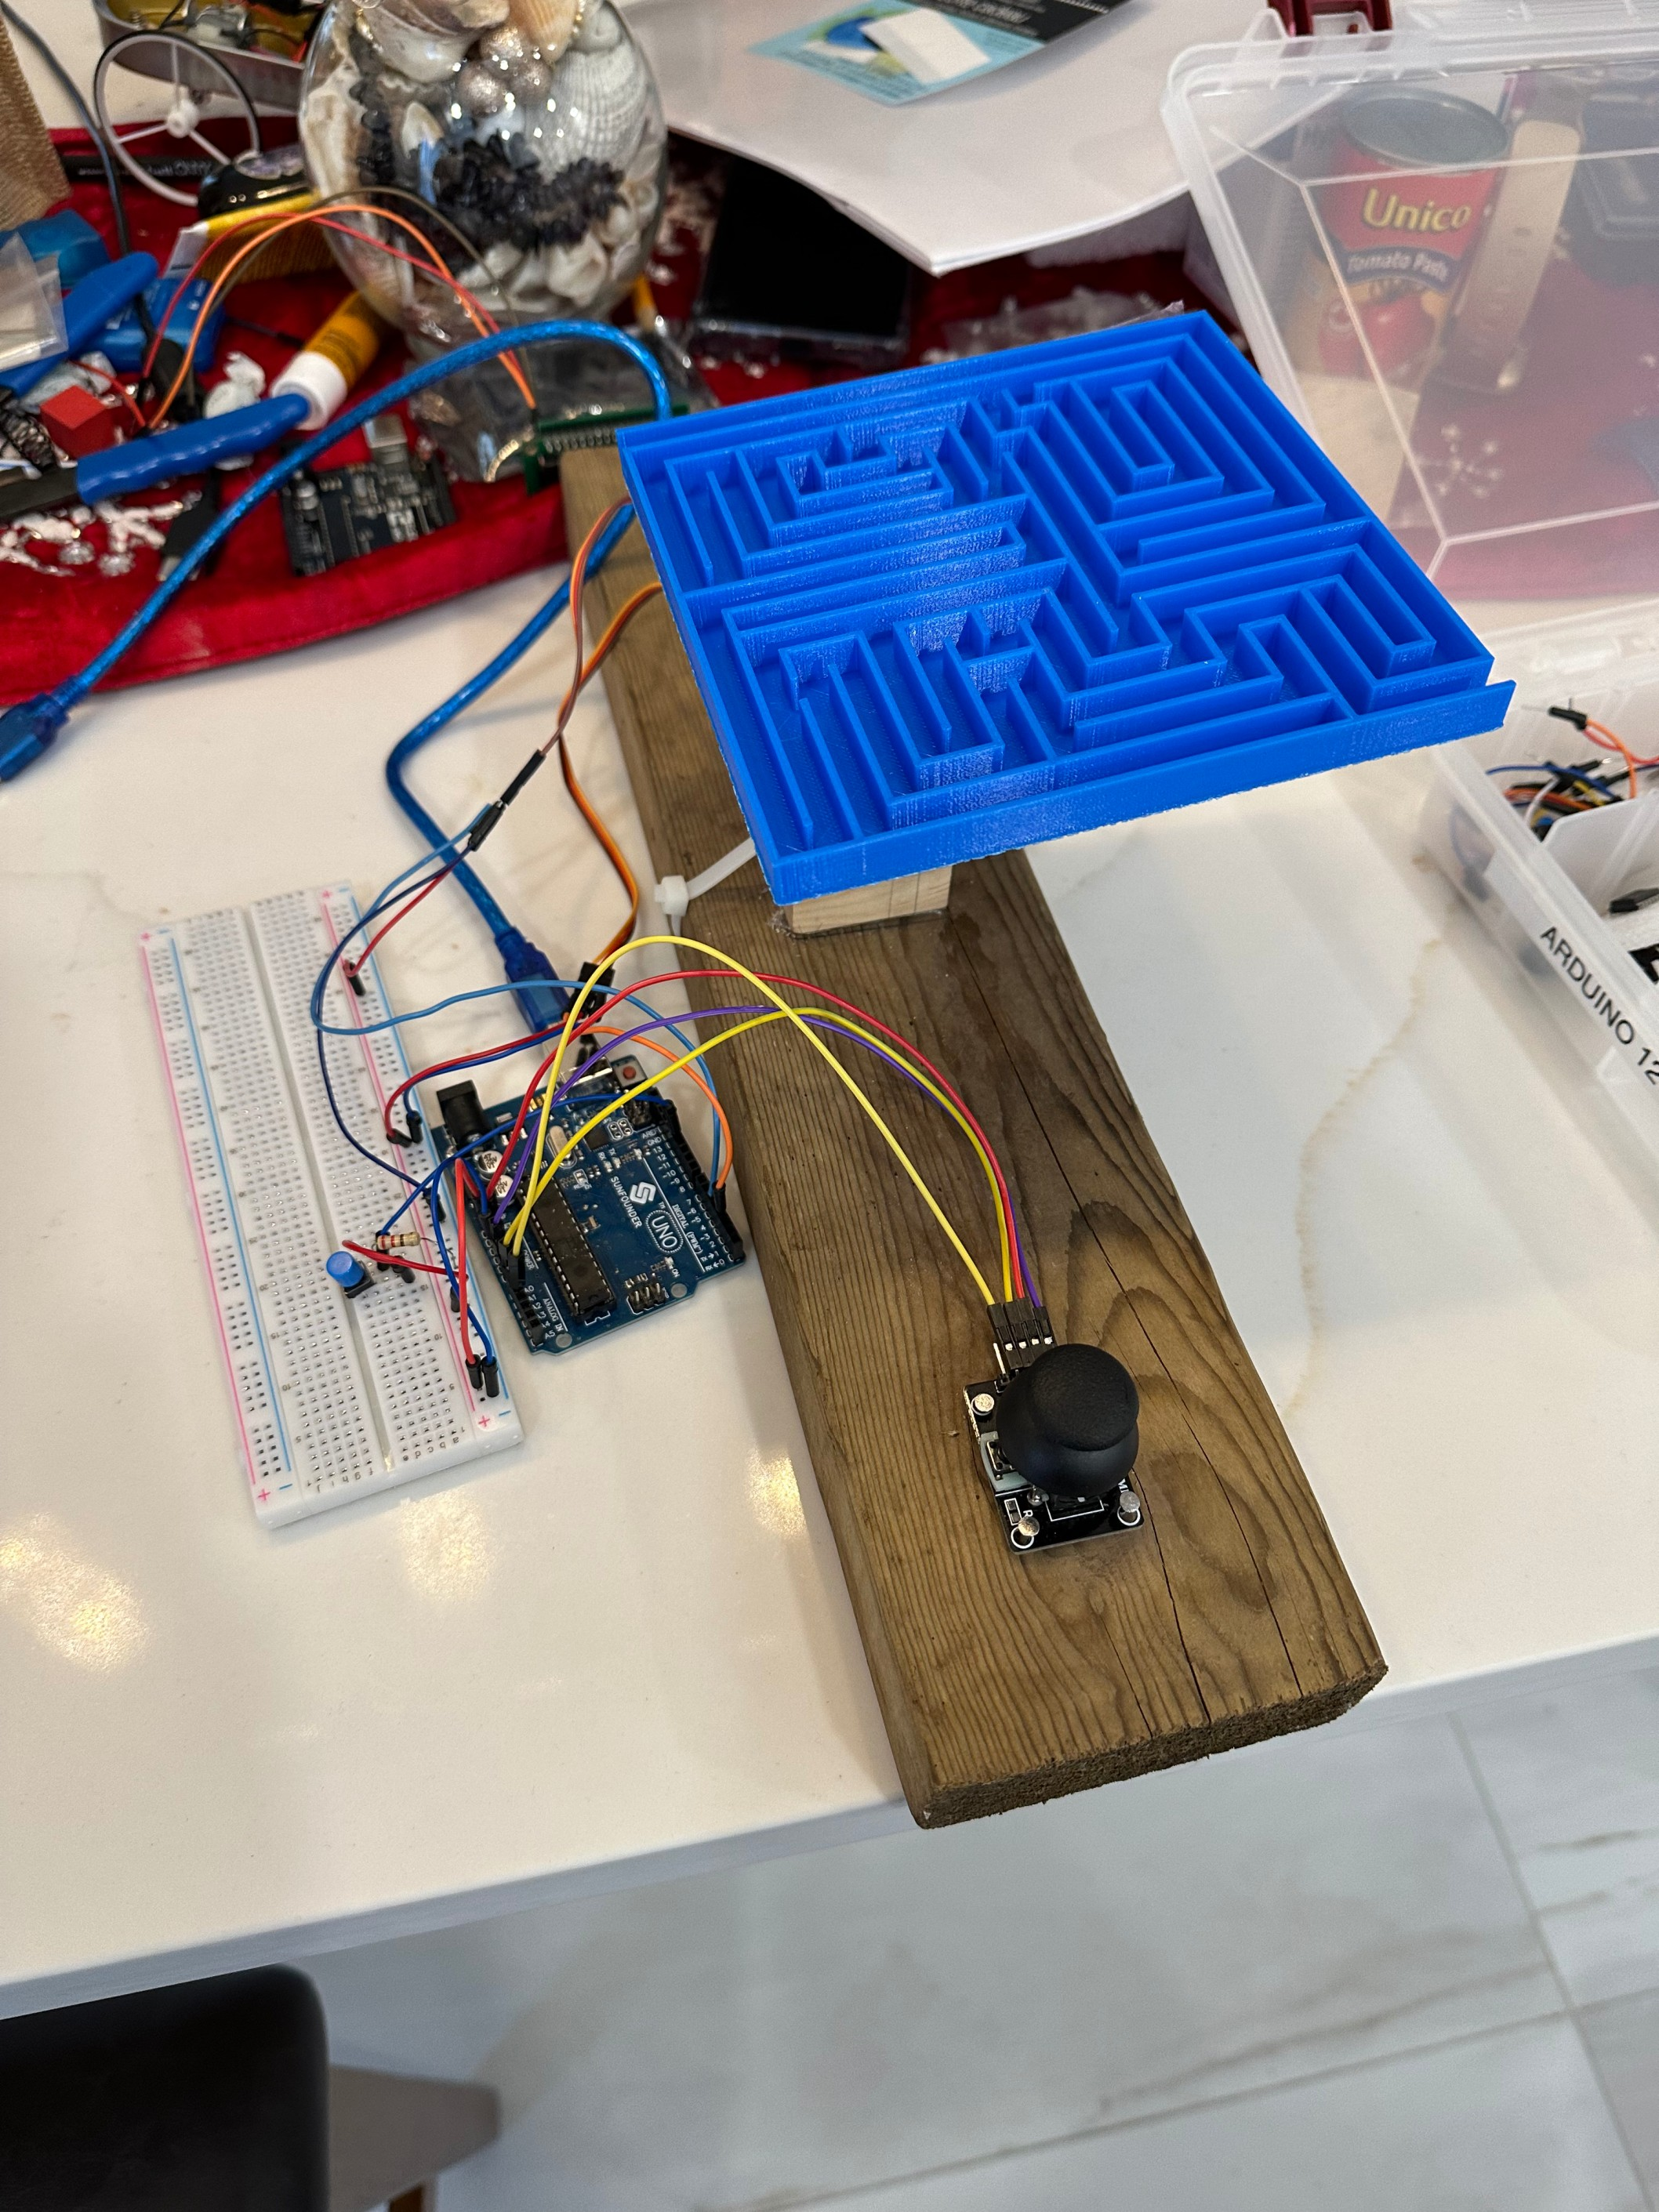
\includegraphics[width=0.7\linewidth]{IMG_0320.jpg}
    \caption{Final Product}
    \label{fig:enter-label}
\end{figure}

\begin{itemize}
    \item Attached the maze structure and joystick to a large wooden plank
    \item Added an additional zip tie through the middle of the small block for added support
  \end{itemize}

\end{document}